\documentclass[tufte-handout]{standalone}
\usepackage{mathpazo} % Sets Palatino as the main font
\usepackage{tikz}
\usetikzlibrary{3d, angles, quotes, calc, backgrounds}
\usetikzlibrary{decorations.markings}
\begin{document}
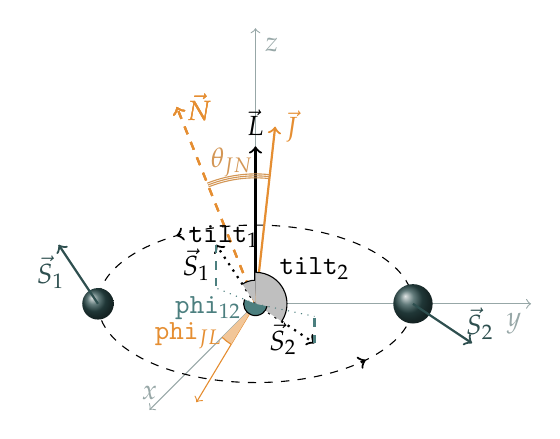
\begin{tikzpicture}[scale=1.]

%my colors
   %my colors
\definecolor{darkslategray}{rgb}{0.18, 0.31, 0.31}
\definecolor{myorange}{rgb}{0.89804, 0.55686, 0.19608}
\definecolor{myorange2}{rgb}{0.82745, 0.58824, 0.33333}
\definecolor{darkslategraylighter}{rgb}{0.29804, 0.49804, 0.49804}
\definecolor{myteal}{rgb}{0.59216, 0.65490, 0.65490}


\definecolor{airforceblue}{rgb}{0.36, 0.54, 0.66}
\definecolor{bittersweet}{rgb}{1.0, 0.44, 0.37}
\definecolor{darkgray}{rgb}{0.66, 0.66, 0.66}
\definecolor{mint}{rgb}{0.24, 0.71, 0.54}

    % Draw the axes
    \def\axisLength{3.5}
    \draw[->,myteal] (0,0,0) -- (\axisLength,0,0) node[anchor=north east] {$y$};
    \draw[->,myteal] (0,0,0) -- (0,\axisLength,0) node[anchor=north west] {$z$};
    \draw[->,myteal] (0,0,0) -- (0,0,\axisLength) node[anchor=south] {$x$};   

    % Origin - center of the orbit
    \coordinate (O) at (0,0);

    % Orbital angular momentum L (vertical)
    \coordinate (L) at (0,2);

    % Defining the positions of the black holes on their elliptical orbit
    % BH1 and BH2 are positioned symmetrically on the ellipse
    \coordinate (BH1) at (-2,0); % Adjust the angle for BH1 position
    \coordinate (BH2) at (2,0); % Adjust the angle for BH2 position

    % Spin vectors S1 and S2 originating from the black holes
    \coordinate (S1) at ($(BH1)+(-0.5,0.75)$);
    \coordinate (S2) at ($(BH2)+(0.75,-0.5)$);
    % Spin coordinates wrt L
    \coordinate (S1_origin) at (-0.5,0.75);
    \coordinate (S2_origin) at (0.75,-0.5);
    % Spin projections onto the orbital plane
    \coordinate (S1_proj) at (-0.5,0.2);
    \coordinate (S2_proj) at (0.75,-0.16);
    
    % Total momentum J (L+S1+S2)
    \coordinate (J) at (0.25,2.25);

    % Line of sight
    \coordinate (N) at (-1, 2.5);
    
    % Draw the elliptical orbit centered at O
    \draw[dashed] (O) ellipse (2cm and 1cm);
    % Give directionality to ellipse
    \draw[->,thick, black] (-0.96,0.877) -- (-1.004,0.865);
    \draw[->,thick, black] (1.337,-0.743) -- (1.4,-0.713);

    % Representing black holes as spheres with distinct dimensions
    \shade[ball color = darkslategray!100] (BH1) circle (0.2cm); % BH1
    \shade[ball color = darkslategray!100] (BH2) circle (0.25cm); % BH2

    % Draw L and J vectors
    \draw[->, thick] (O) -- (L) node[anchor=south] {$\vec{L}$};
    \draw[->, thick, myorange] (O) -- (J) node[anchor=west] {$\vec{J}$};

    % Draw S1 and S2 vectors from the black holes
    \draw[->, thick, darkslategray] (BH1) -- (S1) node[left of = BH1, xshift = 0.4cm, yshift=0.4cm] {$\vec{S}_1$};
    \draw[->, thick, darkslategray] (BH2) -- (S2) node[right of = BH2, xshift=-0.15cm, yshift=-0.25cm] {$\vec{S}_2$};

    % Draw line of sight
    \draw[->,myorange, thick, dashed] (O) -- (N) node[anchor=west] {$\vec{N}$};
    \pic[draw, -, angle eccentricity=1.5, angle radius=1.6cm, color = myorange2] {angle = J--O--N};
    \draw[->,myorange, thick, dashed] (O) -- (N) node[anchor=west] {$\vec{N}$};
    \pic[draw, -, angle eccentricity=1.5, angle radius=1.625cm, color = myorange2] {angle = J--O--N};
    \draw[->,myorange, thick, dashed] (O) -- (N) node[anchor=west] {$\vec{N}$};
    \pic[draw, -, angle eccentricity=1.5, angle radius=1.65cm, color = myorange2] {angle = J--O--N};
    \node[myorange2] at ($(O)+(-0.3,1.8)$) {$\theta_{JN}$};
    % Draw S1 and S2 with respect to L
    \draw[->,black,thick, dotted] (O) -- (S1_origin) node[left of = S1_origin, xshift=0.75cm, yshift=-0.25cm] {$\vec{S}_1$};
    \draw[->,black,thick, dotted] (O) -- (S2_origin) node[right of = S2_origin, xshift=-1.4cm, yshift=0.05cm] {$\vec{S}_2$};

    
    % tilt angles
    \pic[draw, -, angle eccentricity=1.5, angle radius=0.3cm, color = black, fill = lightgray] {angle = L--O--S1_origin};
    \node at ($(O)+(-0.4,0.85)$) {\texttt{tilt}$_1$};
    \pic[draw, -, angle eccentricity=1.5, angle radius=0.4cm, color = black, fill = lightgray] {angle = S2_origin--O--L};
    \node at ($(O)+(0.75,0.45)$) {\texttt{tilt}$_2$};

    % Project S1 and S2 onto the orbital plane

    
    % phi angles
    %\pic[draw, -, angle eccentricity=1.2, angle radius=1.5cm, color = myorange] {angle = J--O--L};
    %\pic[draw, -, angle eccentricity=1.2, angle radius=1.45cm, color = myorange] {angle = J--O--L};
    %\node[myorange] at ($(O)+(0.75,1.6)$) {\texttt{phi}$_{JL}$};
    \coordinate (Jproj) at (-0.75, -1.25);
    \coordinate (xAxis) at (0, 0, \axisLength);
    \draw[->, solid, myorange] (O) -- (Jproj);
    % phi angles
    \pic[draw, -, angle eccentricity=1.2, angle radius=0.6cm, color = myorange, fill = myorange!50] {angle = xAxis--O--Jproj};
    \node[myorange] at ($(O)+(-0.85,-0.4)$) {\texttt{phi}$_{JL}$};

    \draw[-,thick, darkslategraylighter, dashed] (S1_origin) -- (S1_proj);
    \draw[-,thick, darkslategraylighter, dashed] (S2_origin) -- (S2_proj);

    \draw[-, darkslategraylighter, dotted] (O) -- (S1_proj);
    \draw[-, darkslategraylighter, dotted] (O) -- (S2_proj);
    \pic[draw, -, angle eccentricity=1.2, angle radius=0.15cm, color = black, fill = darkslategraylighter] {angle = S1_proj--O--S2_proj};
    \node[darkslategraylighter] at ($(O)+(-0.6,-0.05)$) {\texttt{phi}$_{12}$};
    
\end{tikzpicture}
\end{document}